\documentclass{article}
\usepackage[utf8]{inputenc}

\usepackage{geometry}

\usepackage{fancyhdr}
% \usepackage{fullpage}
\usepackage{lscape}

% \usepackage{booktabs}
% \usepackage{verbatim}

% \usepackage{algpseudocode}
% \usepackage{algorithm}

% \usepackage{amsmath, amsfonts, amsthm, bm}
% \usepackage{hyperref}
% \usepackage{cleveref}

\usepackage{tikz}
\usetikzlibrary{backgrounds,decorations.pathreplacing}
\usetikzlibrary{calc}
\usetikzlibrary{matrix}
\usetikzlibrary{backgrounds}
\usetikzlibrary{shapes}
\usetikzlibrary{positioning}

\usepackage{graphicx}
\usepackage{subcaption}

% \usepackage[inline]{enumitem}

% \usepackage{todonotes}
% \usepackage[framemethod=tikz]{mdframed}

\newcommand\grid[1]{
  \pgfmathsetmacro\size{#1}
  \draw[step=1,black,thin] (0,0) grid (\size-1,\size-1);
  \draw[step=\size-1,black,ultra thick] (0,0) grid (\size-1,\size-1);
}

\newcommand\xlabels[2]{
  \foreach \label [count=\i] in #2 {
    \node at (\i-1,-0.5) {\texttt{\label}};
    \node at (\i-1,#1-0.5) {\texttt{\label}};

    \ifnum \i=#1
      \breakforeach
    \fi
  }
}

\newcommand\ylabels[2]{
  \foreach \label [count=\i] in #2 {
    \node at (-0.5,#1-\i) {\texttt{\label}};
    \node at (#1-0.5,#1-\i) {\texttt{\label}};

    \ifnum \i=#1
      \breakforeach
    \fi
  }
}

\newcommand\upperlabels{A,...,Z}
\newcommand\lowerlabels{do,re,mi,fa,so,la,si}
\newcommand\numberlabels{1,...,19}

\newcommand\upperboard[1]{
  \grid{#1}
  \xlabels{#1}{\numberlabels}
  \ylabels{#1}{\lowerlabels}
}

\newcommand\numberboard[1]{
  \grid{#1}
  \xlabels{#1}{\lowerlabels}
  \ylabels{#1}{\upperlabels}
}

\newcommand\lowerboard[1]{
  \grid{#1}
  \xlabels{#1}{\upperlabels}
  \ylabels{#1}{\numberlabels}
}

\title{Multiverse Go}
% \author{}
\date{}

\begin{document}
\maketitle

\pagestyle{empty}

\section{Rules}

Multiverse go is a variant similar but distinct from 3D go.  Like 3D go, it is
played on a 3D goban.  However, the rules concerning stone liberties are
different.
%
The game is played on a 3D goban;  in this document we will use the $5\times
5\times 5$ grid as an example.  Rather than seeing it as a single $5 \times
5\times$ game of go, it should be seen as $15$ separate (but connected)
$5\times 5$ games.  Each 2D ``slice'' of the 3D goban represents a separate
``flat'' game.  In practice, when each move in the $5\times 5\times 5$ goban
corresponds to $3$ moves and $12$ passes in the $5\times 5$ ``slice'' gobans.

Each intersection can be identified by using 3D coordinates which range from
$\texttt{A1a}$ to $\texttt{E5e}$.  These coordinates can be used to uniquely
identify both the 2D ``slice'' gobans in which the moves are being played, and
the coordinates within those ``slice'' gobans.
%
Each 2D board has a unique name;  in $5\times 5\times 5$ multiverse go, the
names are 
%
\texttt{A}, \texttt{B}, \texttt{C}, \texttt{D}, \texttt{E},
%
\texttt{1}, \texttt{2}, \texttt{3}, \texttt{4}, \texttt{5},
%
\texttt{a}, \texttt{b}, \texttt{c}, \texttt{d}, and \texttt{e}.
%
As an example, move \texttt{B4c} represents three moves:
%
\begin{itemize}
  %
  \item Move \texttt{4c} on board \texttt{B};
  %
  \item Move \texttt{Bc} on board \texttt{4};
  %
  \item Move \texttt{B4} on board \texttt{c};
  %
\end{itemize}

\newgeometry{margin=0cm,includeheadfoot}

\begin{center}
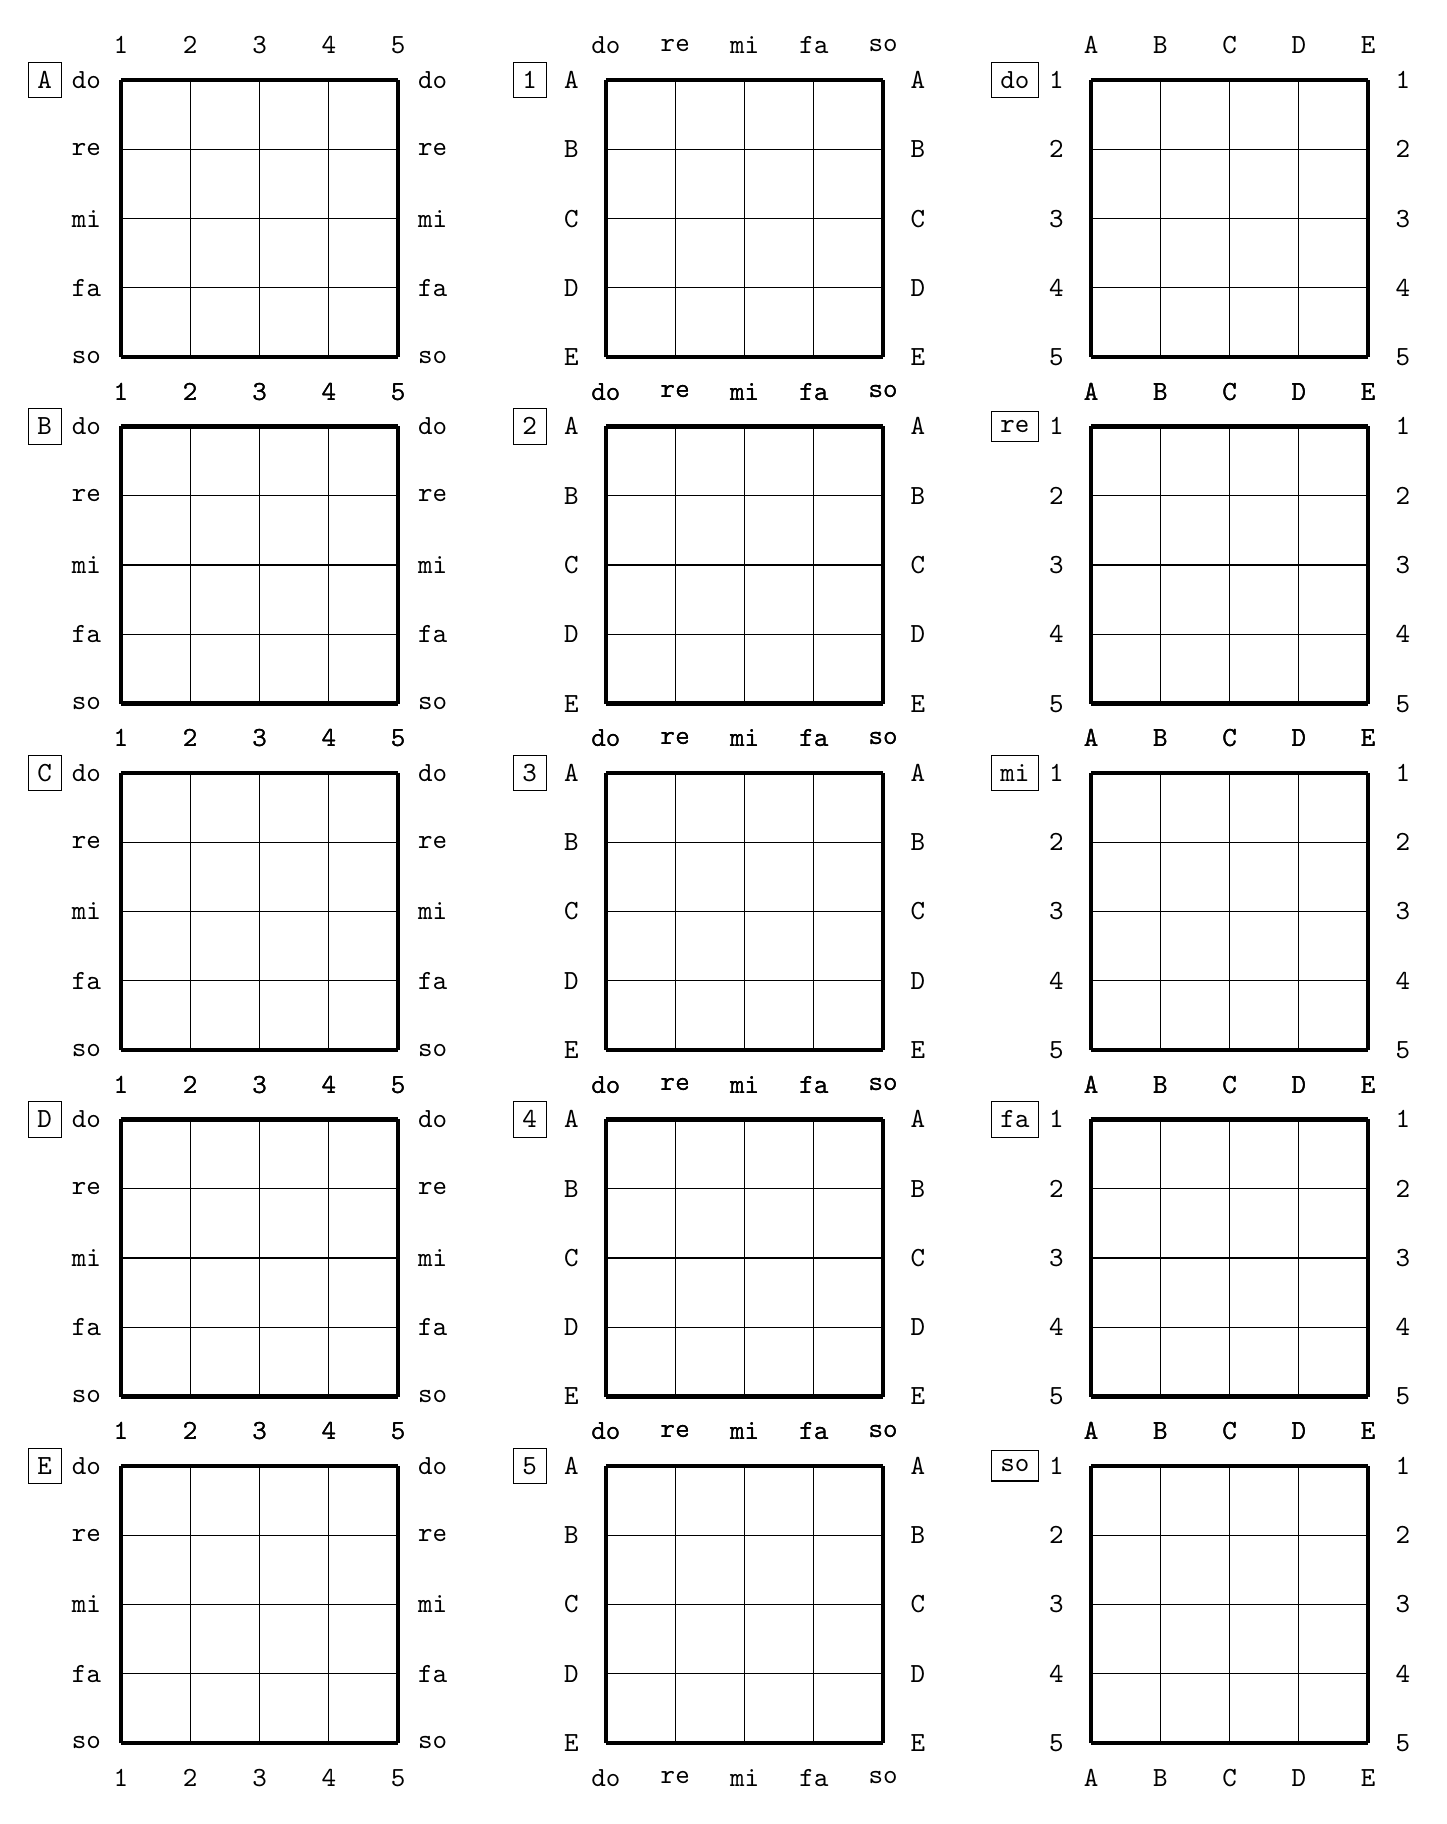
\begin{tikzpicture}
  %
  \newcommand\size{5}
  \begin{scope}[scale=1.1]

    \foreach \name [count=\i] in \upperlabels {
      \begin{scope}[scale=0.8,yshift=-\i*\size cm]

        \begin{scope}[shift={(-1.1,\size - 1)}]
          \node[draw] at (0,0) {\texttt{\name}};
        \end{scope}

        \upperboard{\size}

        \ifnum \i=\size
          \breakforeach
        \fi

      \end{scope}
    }

    \foreach \name [count=\i] in \numberlabels {
      \begin{scope}[scale=0.8,yshift=-\i*\size cm,xshift=7cm]

        \begin{scope}[shift={(-1.1,\size - 1)}]
          \node[draw] at (0,0) {\texttt{\name}};
        \end{scope}

        \numberboard{\size}

        \ifnum \i=\size
          \breakforeach
        \fi

      \end{scope}
    }

    \foreach \name [count=\i] in \lowerlabels {
      \begin{scope}[scale=0.8,yshift=-\i*\size cm,xshift=14cm]

        \begin{scope}[shift={(-1.1,\size - 1)}]
          \node[draw] at (0,0) {\texttt{\name}};
        \end{scope}

        \lowerboard{\size}

        \ifnum \i=\size
          \breakforeach
        \fi

      \end{scope}
    }

  \end{scope}

\end{tikzpicture}
\end{center}

\begin{center}
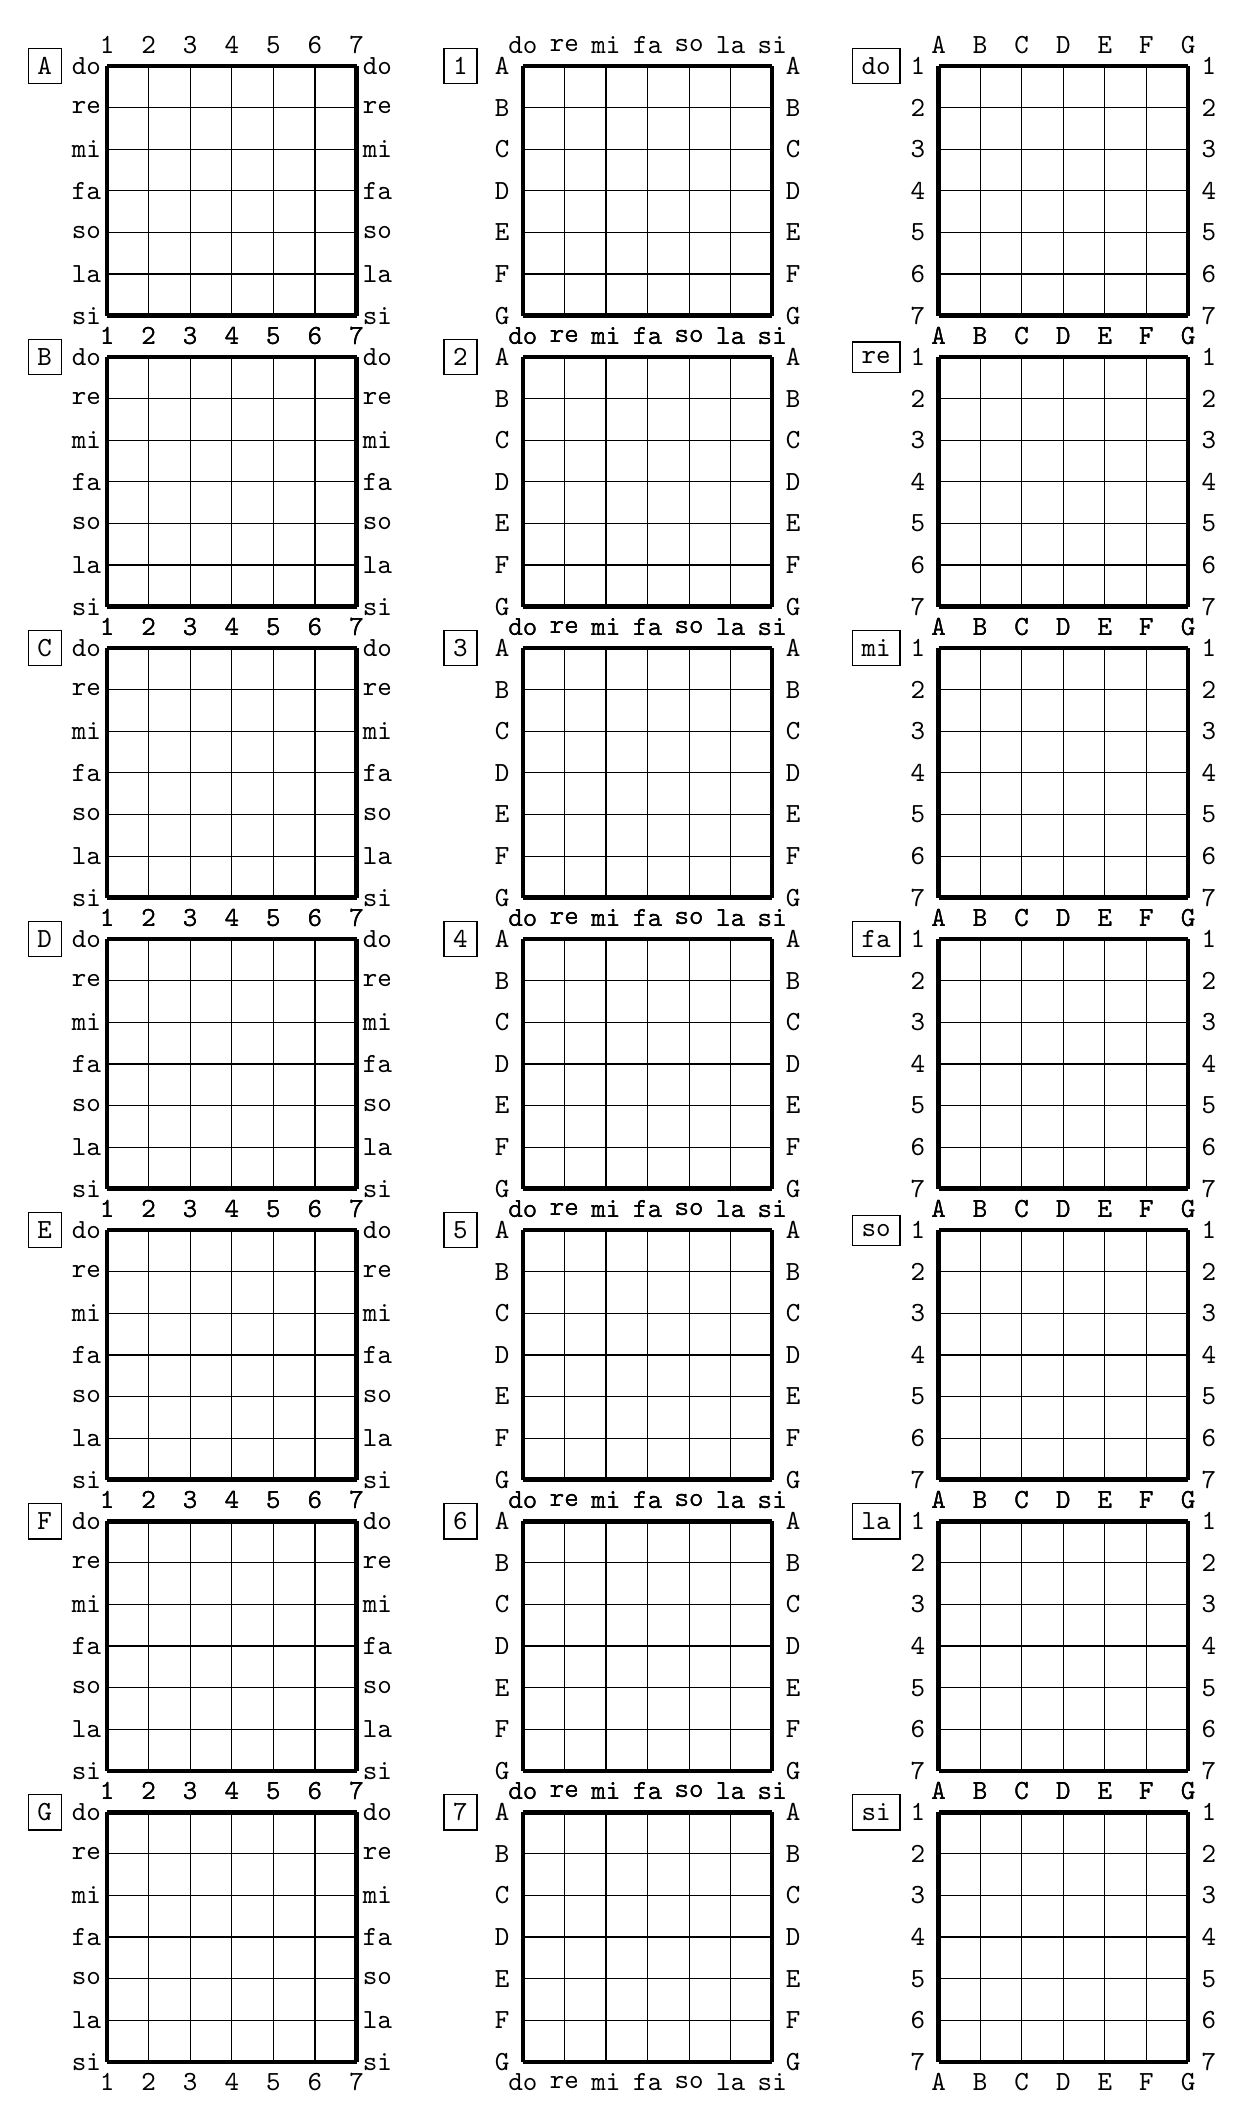
\begin{tikzpicture}
  %
  \newcommand\size{7}
  \begin{scope}[scale=0.66]

    \foreach \name [count=\i] in \upperlabels {
      \begin{scope}[scale=0.8,yshift=-\i*\size cm]

        \begin{scope}[shift={(-1.5,\size - 1)}]
          \node[draw] at (0,0) {\texttt{\name}};
        \end{scope}

        \upperboard{\size}

        \ifnum \i=\size
          \breakforeach
        \fi

      \end{scope}
    }

    \foreach \name [count=\i] in \numberlabels {
      \begin{scope}[scale=0.8,yshift=-\i*\size cm,xshift=10cm]

        \begin{scope}[shift={(-1.5,\size - 1)}]
          \node[draw] at (0,0) {\texttt{\name}};
        \end{scope}

        \numberboard{\size}

        \ifnum \i=\size
          \breakforeach
        \fi

      \end{scope}
    }

    \foreach \name [count=\i] in \lowerlabels {
      \begin{scope}[scale=0.8,yshift=-\i*\size cm,xshift=20cm]

        \begin{scope}[shift={(-1.5,\size - 1)}]
          \node[draw] at (0,0) {\texttt{\name}};
        \end{scope}

        \lowerboard{\size}

        \ifnum \i=\size
          \breakforeach
        \fi

      \end{scope}
    }

  \end{scope}

\end{tikzpicture}
\end{center}

\end{document}
